
\documentclass[a4paper]{article}
\usepackage{graphicx}
\begin{document}
	\begin{center}{\Huge \centering  Smart Radar }
			\end{center}
	{\fontsize{10}{12} Martina Cavallucci  765565
		\newline Matteo Magnini      731659
		\newline Alfredo Tonelli 759161
		\newline Shapour Nemati -----------
	}
	
	\section{Architettura e funzionamento del sistema}
	   
	\begin{figure}[!htb]
		\centering
			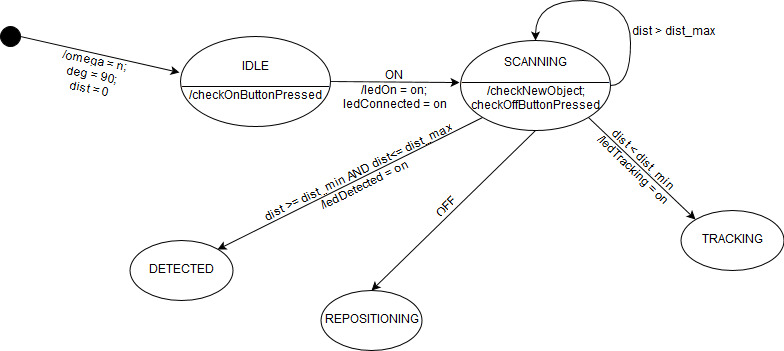
\includegraphics[scale=0.5]{figura1.jpg}
		\caption{IDLE-SCANNING}
	\end{figure}

In figura 1 sono descritti lo stato di IDLE  e quello di SCANNING. Infatti quando il sistema si avvia parte dallo stato di IDLE e il servo si trova ad un\newline angolo di 90$^{\circ}$; se il bottone ON viene premuto allora il Radar simulato da tutta la parte di Arduino inzia lo SCANNING con una certa "delta" velocita' e \newline vengono accesi i ledON e il ledConnected. \newline
Il sistema inizia a scandagliare l'ambiente finche' non si verifica uno dei tre seguenti casi :
\begin{itemize}
	\item Rileva un oggetto nel suo campo di azione che va da DIST-MIN a DIST-MAX cosi' accende il ledDetected e passa allo stato DETECTED
	\item Rileva un oggetto troppo vicino al sensore (distanza rilevata minore della DIST-MIN) cosi' si accende il ledTracking e passa allo stato TRACKING 
	\item Il bottone OFF viene premuto e si passa allo stato di REPOSITIONING
\end{itemize}

	\newpage
	
	\begin{figure}[!htb]
		\centering
		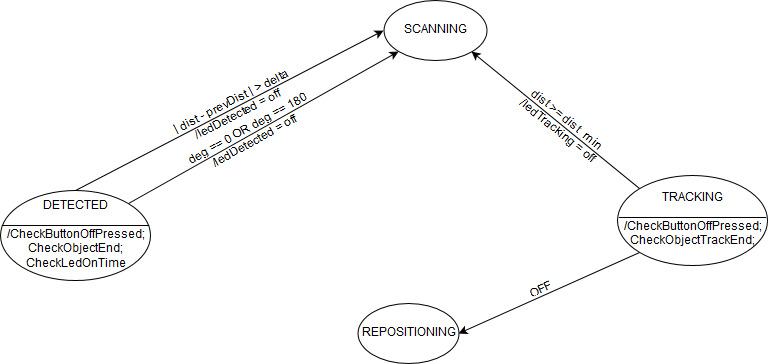
\includegraphics[scale=0.6]{figura2.jpg}
		\caption{DETECTED-TRACKING}
	\end{figure}


	In figura 2 sono descritti nel dettaglio lo stato DETECTED e lo stato TRACKING.
	All'interno dello stato DETECTED viene controllato se la differenza tra la distanza corrente e la distanza precedente e' maggiore di un certo delta fissato da noi per capire se un oggetto è "finito" allora il ledDetected viene spento e si torna allo stato di SCANNING; inoltre anche se si arriva ai limiti di movimeno del servo si ritorna allo stato di SCANNING.
	All'interno dello stato TRACKING,invece, controllo se l'oggetto non viene piu' rilevato come troppo vicino e quindi torno allo stato di SCANNING oppure controllo se viene premuto il bottonOff e passo allo stato di REPOSITIONING il quale si occupera' di riposizionare il servo e di resettare alcune variabili significative.

	\newpage
	\begin{figure}[!htb]
		\centering
		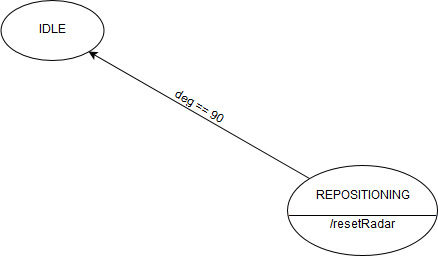
\includegraphics[scale=0.8]{figura3.jpg}
		\caption{REPOSITIONING}
	\end{figure}
	\vskip .5truecm 

In figura 3 si descrive lo stato di REPOSITIONING nel quale resetto l'angolazione a 90$^{\circ}$ e comunico ad Arduino l'angolazione che il servo deve tenere.



	\section{Guida utente}
	.................

\end{document}